% !TeX root = ../main.tex
% Add the above to each chapter to make compiling the PDF easier in some editors.

\chapter{Fake News Detection Models}\label{chapter:fnd_models}
The automated detection of fake news on social media comes with its characteristic challenges. First, the fact
that fake news are constructed to misguide its consumers makes them hard to distinguish by only using news content. Second, when we include social context into the model, the large-scale and noisy nature of social context data represents another issue~\parencite{HierarchicalPropagationNetworksForFND_Shu}. Moreover, from a broader perspective, fake news should be detected before it becomes widespread so that the amount of users affected can be minimized.\\
In this chapter, we examine how these challenges effect the model and dataset's design. We initially take a look at news content models in section~\ref{sec:newsContentModels}. In first section, we lay out the definitions for the materials used. After we give a detailed analysis of the dataset, we talk about the tokenizer and model itself, discuss its performance on the dataset. In section~\ref{sec:socialContextModels} we investigate social context based and hybrid models. Similar to the first section, we give definitons for the used material, then talk about the dataset and model. In this section, we also examine issues such as early fake news detection and model aging.\\

\section{News Content Models}
\label{sec:newsContentModels}
The majority of approaches for FND models utilizes news content. Models that base their predictions only on news content focus on the patterns in the text, especially words or word groups that appear frequently in other instances of the same class. As discussed in Section~\ref{sec:fakeNewsDetection}, there exist a variety of approaches available for news content models, however, due to unavailable or outdated datasets, we were unable to work with most news content models.

\subsection{Notation and Definitions}
\label{subsec:newsContentModels_Definitions}
Here we introduce the notation utilized in this section. Note that these notations will appear in its context, which will provide concrete examples for each symbol defined in Table~\ref{tab:newsContentModels_Notation}.\\
\begin{table}
    \begin{tabular}{cp{0.8\textwidth}}
        $x^{raw}$       & Input news article.                                            \\
        $y^{raw}$       & The label of news article.                                     \\
        $T$             & Tokenizer function                                             \\
        $\psi$          & Label mapping function                                         \\
        $x^{tok}$       & Tokenized news article                                         \\
        $y$             & Vectorized class value.                                        \\
        $|x^{tok}|$     & The number of tokens in $x^{tok}$.                             \\
        $X^{raw}$       & The space of $x^{raw}$                                         \\
        $X^{tok}$       & The space of $x^{tok}$.                                        \\
        $Y^{raw}$       & The space of $y^{raw}$                                         \\
        $Y$             & The space of $y$                                               \\
        $p$             & Position of a token in the tokenized article $x^{tok}$.        \\
        $x^{tok}_p$     & A token at position $p$ of the tokenized article $x^{tok}$     \\
        $V$             & Vocabulary: A collection of tokens available to the tokenizer. \\
        $f$             & Classifier function, i.e., FND model.                          \\
        $y^*$           & Prediction of FND model.                                       \\
        $x$             & Numeric vector of $x^{tok}$                                    \\
        $X$             & Space of $x$                                                   \\
        $f(x)_y$        & Prediction score for class $y$ given input $x$                 \\
        $l$             & Index of a layer                                               \\
        $l_{embedding}$ & Embedding layer                                                \\
        $a_{i}^{(l)}$   & The value of unit $i$ in layer $l$                             \\
        $w_{ij}^{(l)}$  & Weight between units $i$ in layer $l$ and $j$ in layer $l+1$   \\
        $\sigma$        & Activation function                                            \\
        $L$             & Loss function                                                  \\
    \end{tabular}
    \caption[Notation]{Notation used in this section.}
    \label{tab:newsContentModels_Notation}
\end{table}
Using this notation we now define some relevant concepts. First, we talk about terms and definitions for \emph{tokenization}, illustrate the mathematical insight in the tokenization process. First, to build upon a concrete foundation, let us consider a news article $x^{raw}$ fed to the tokenizer.
\begin{definition}[\emph{Tokenizer}]
    A tokenizer $T:X^{raw} \mapsto X^{tok}$ is a function that maps raw textual data to smaller units called tokens.
\end{definition}
A token can be a word, character or a subword. Therefore, we define three types of tokenization techniques:
\begin{itemize}
    \item \emph{Word tokenization} splits the given text into individual words based on a delimeter such as whitespace, commma, etc. This approach creates a vocabulary (V) from the inputs it was trained on. All words do not appear in the vocabulary are replaced with unknown token ([UNK]), and this concept is called being \emph{Out Of Vocabulary}(OOV). Depending on the task, the size of the vocabulary can grow quite large. The solution for exploding vocabulary sizes was introduced in subword tokenization. The commonly used examples for word tokenizers are Word2Vec~\parencite{Word2Vec_Mikolov} and GloVe~\parencite{GloVe_Pennington}.
    \item \emph{Character tokenization} splits the text into single characters. Since the size of available characters is limited and known, the OOV problem is solved by encoding the unknown word by means of its characters. Although looks like a good solution, the length of tokens can be massive for long texts.
    \item \emph{Subword tokenization} splits the given text into subwords, also called \emph{n-gram characters}. For instance, comparative words like harder is segmented into hard-er, or superlative words like hardest is segmented into hard-est. The most common method for subword tokenization is \emph{Byte Pair Encoding} (BPE). BPE was introduced by~\cite{ANewAlgorithmForDataCompression_Gage} but adapted to word segmentation by~\cite{NeuralMachineTranslationOfRareWords_Sennrich}. BPE iteratively merges the most frequently appearing character or character sequences. This approach allows for an efficient space usage thus smaller vocabularies~\parencite{NeuralMachineTranslationOfRareWords_Sennrich}.
\end{itemize}
We say that an input is \emph{tokenized} after it is fed to the tokenizer. A tokenized news article $x^{tok} \in X^{tok}$ is a vector of tokens in which the order of the words and characters in $x^{raw} \in X^{raw}$ are kept.
\begin{center}
    $T(x^{raw}) = x = [x_1, x_2, \dots, x_n]$, where $n = |x|$.
\end{center}
We denote an element of $x^{tok}$ at $p$-th position as $x_p^{tok}$, and the number of tokens in $x^{tok}$ as $|x^{tok}|$. Thus, we have the range of p, $1 \leq p \leq |x^{tok}|$. The tokens
Furthermore, we denote the space of raw label $Y^{raw} = \{"fake", "real"\}$, with
$y^{raw} \in Y^{raw}$. We use a label mapping function $\psi: Y^{raw} \mapsto Y$ that maps raw labels to classes, where $Y \in \mathbb{R}^2$ with,
\begin{center}
    \[\psi(y^{raw}) = y =
        \begin{cases}
            0, & y^{raw} = "fake" \\
            1, & y^{raw} = "real"
        \end{cases}
    \]
\end{center}
In order to feed the input to the model, we need numeric data which can be obtained by numerous techniques. One widely used approach is BoW representation which produces features based on the number of occurrences of a word or token. An alternative BoW representation uses the presence/absence of word instead of frequencies. A more sophisticated approach is \emph{Word2Vec}, which encodes words into numeric values by learning word associations. From the perspective of representation of a word, \emph{Word2Vec} can capture different degrees of similarity between words which allows for preservation of semantic and syntactic relationships~\parencite{Word2Vec_Mikolov}. It is clear that the transformation of words into numeric vectors is a very crucial stage for FND since we need to maintain as much contextual information as possible. Yet, the SOTA is an even more sophisticated approach called \emph{Transformer} which is utilized by many language models such as BERT. We will discuss Transformer architecture in~\ref{subsec:newsContentModels_TransformerArch}. For ease of the notation, we refer to this stage as \emph{Embedding Layer} and denote it with $l_{embedding}$.\\
The input transformation pipeline is illustrated in~\ref{fig:InputPreProcessPipeline}.
\begin{figure}
    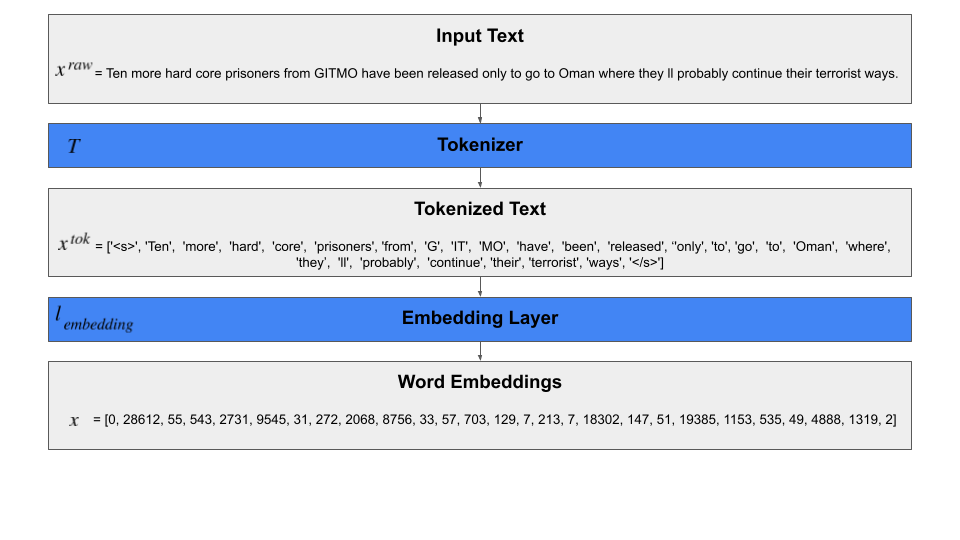
\includegraphics[scale=0.43]{InputPreProcessPipeline.png}
    \caption[The preprocessing pipeline for a textual input.]{The preprocessing pipeline for a textual input.}
    \label{fig:InputPreProcessPipeline}
\end{figure}
\begin{definition}[\emph{FND Classifier}]
    An FND classifier $f:X \mapsto Y$ is a function that outputs a predicted scores $f(x)_y$ for each class $y$ for a given input $x$.
\end{definition}
\begin{definition}[\emph{Prediction}]
    A prediction $y^*$ is the maximum of predicted scores $f(x)_y$ of an FND classifier.
    \begin{center}
        $y^* = argmax_{y \in Y} f(x)_y$
    \end{center}
\end{definition}
\begin{definition}[\emph{FND Neural Network Classifier}]
    A neural network classifier is a \emph{classifier} $f$ that comprises of layers $l$ with $1 \leq l \leq L$, where $L$ denotes the number of layers. Each layer has a set of units $a_i^{(l)}$ with $i$ denoting the position of the unit in
    a layer $l$. We say that between two units $a_i^{(l)}$ belonging to layer $l$ and $a_j^{(l+1)}$ belonging to layer
    $l+1$ have a weight value $w_{ij}^{(l)}$ that connects them. Along with a non-linear activation function $\sigma$, we
    can define the value of the $j$-th unit $a_j^{(l+1)}$ in terms of weights and unit values from previous layer for an FCN, with $N$ is the number of units in layer $l$.
    \begin{center}
        $a_j^{(l+1)} = \sigma(\sum_{i=1}^{N} a_i^{(l)} w_{ij}^{(l)})$
    \end{center}
\end{definition}
\begin{figure}
    \centering
    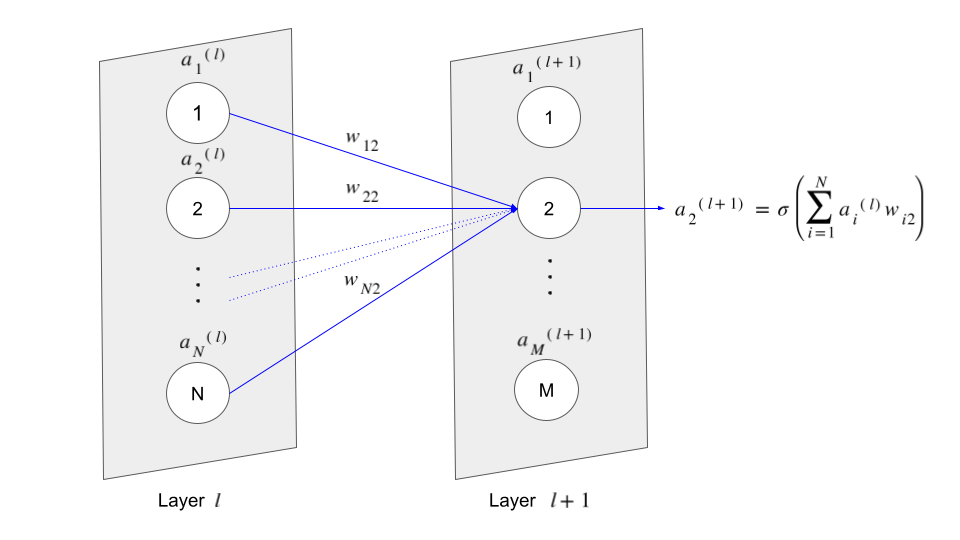
\includegraphics[scale=0.43]{NN_LayerRepresentation}
    \caption[Units and layers of an FCN]{Units and layers of an FCN. For brevity, arrows and weights are only drawn for $a_2^{(l+1)}$}
    \label{fig:NN_LayerRepresentation}
\end{figure}
Neural networks iteratively optimize the weights between layers such that the produced output is as close as to the
expected output. This is done so using optimization methods such as \emph{Gradient Descent} (GD)~\parencite{GD_Cauchy},
\emph{Stochastic Gradient Descent} (SGD)~\parencite{SGD_Robbins}, \emph{Adaptive Moment Estimation} (Adam)~\parencite{Adam_Kingma} to minimize the loss function $L$. While there exist many optimization methods available for nueral networks, we do not examine any of them.\\
For classification problems, we adopt a layer called \emph{Softmax}~\parencite{Softmax_Bridle} outputs the predicted scores $f(x)_y$ for each class $y$ by normalizing outputs $Z_y(x)$ from the previous layer.\\
\begin{center}
    $f(x)_y = \dfrac{exp(Z_y(x))}{\sum_{\hat{y} \in Y} exp(Z_{\hat{y}(x)})}$
\end{center}
The FCNs are the simplest architectures for neural networks. In an FCN, all units are connected which means there is a weight between each unit in layer $l$ and $l+1$. While very simple to construct, usage of these architectures when modeling sequences is not preferred due to the number of trained parameters such as weights and biases. Instead, when modeling sequences like sentences and documents, a common approach is RNNs which allow previous outputs to be used while having hidden states. However, RNNs are not powerful enough to represent long-term dependencies~\parencite{LearningLongTermDependenciesHard_Bengio} and suffer from vanishing/exploding gradients~\parencite{OnTheDifficultyOfTrainingRNNs_Pascanu}. Utilizing RNNs, an idea was proposed in which these shortcomings were addressed. Called \emph{Long Short-Term Memory} (LSTM)~\parencite{LSTM_Hochreiter}, the idea is to keep a cell state which is updated with previous cell's state. This cell state is conveyed to the consequent cells to form a chain that represents the document. More precisely, each cell corresponds to a token whose information will be shared with consequent tokens by the propagation of previously mentioned cell states. This approach is indeed very useful for long documents since news articles tend to be long and their sentences contextually relevant. LSTM is usually used in different variations based on the same idea. For instance, a consequent study has extended LSTMs with \emph{peephole connections} in~\parencite{LSTMPeephole_Gers}. LSTMs have been proven to deliver a good performance in NLP tasks such as \emph{speech recognitions}~\parencite{AchievingHumanParityinConvSR_Wayne}.\\
LSTMs perform well however due to long training times and large memory requirements during training, they are being replaced with attention-based models. Having introduced all necessary notation and definitions, in ~\ref{subsec:newsContentModels_TransformerArch}, we discuss the SOTA approach the Transformer models which are based on attention mechanism.

\subsection{Transformer Architecture}
\label{subsec:newsContentModels_TransformerArch}
Transductive learning has been successfully utilized along with encoder-decoder structure in many language
tasks~\parencite{S2SLearningWithNNs_Sutskever, LearningPhraseRepresentations_Cho, AttentionIsAllYouNeed_Vaswani}. Transduction is first proposed in~\cite{LearningByTransduction_Gammerman} to counteract with unlabeled data problem.
In contrast to supervised learning, transductive learning does not require all data to be labeled, instead it utilizes
the clustered behavior of data. Using the gaps between different clusters and a small set of labeled data, transductive learning assigns labels to unlabeled data. Accordingly, Transformer models are transductive models and use encoder-decoder structure to achieve that.\\
Encoder-decoder structure that takes into account the order of words was proposed in~\parencite{LearningPhraseRepresentations_Cho}. This encoder-decoder structure consists of one RNN as encoder and one RNN as decoder. The encoder maps an input sequence to fixed-length vector, and the decoder maps this fixed-length vector to a target sequence. Transformer architecture adopts a similar approach which employs feed-forward and Multi-Head Attention layers in both encoder and decoder which is illustrated in Fig.~\ref{fig:transformerArchitecture} with N=6 stacks of encoders and decoders.\\
In order to reduce sequential computation, CNNs have been adopted as building blocks that parallelly compute hidden representations for all input and output positions~\parencite{AttentionIsAllYouNeed_Vaswani}. Although aimed to reduce computation, the number of operations to convey information from one random input or output to another increases linealy in ByteNet~\parencite{ByteNet_Kalchbrenner} and logarithmically in ConvS2S~\parencite{ConvS2S_Gehring}. Contrary to CNNs, Transformers are able to fix the number of operations by averaging attention-weighed positions which decreases the effective resolution. However, this decrease in resolution is neutralized by the utilization of Multi-Head Attention~\parencite{AttentionIsAllYouNeed_Vaswani}.
\begin{figure}
    \centering
    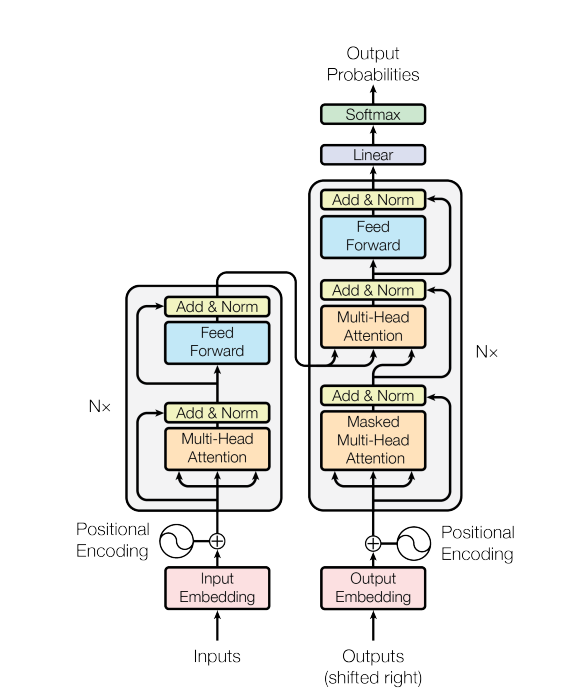
\includegraphics{TransformerArchitecture.png}
    \caption[The Transformer Model Architecture]{The Transformer Model Architecture (N=6). Figure obtained from~\parencite{AttentionIsAllYouNeed_Vaswani}}
    \label{fig:transformerArchitecture}
\end{figure}
Initially suggested in the decoder of the model proposed in~\parencite{NeuralMachineTranslationByJointlyLearning_Bahdanau}, an attention mechanism works similar to human attention; it learns to put more importance on some words that convey the relevant information about the sentence. It does so by means of a context vector that depends on a sequence of \emph{annotations}. An annotation $h_i$ for a word (or embedding) $x_i$ contains information about the complete input sentence but with a focus on the words that are closer to the word $x_i$. The context vector $c_i$ for word $x_i$ is obtained as a weighted sum of all these annotations $h_i$:
\begin{center}
    $c_i = \sum_{j=1}^{|x|} \alpha_{ij} h_j$.
\end{center}
The weight $\alpha_{ij}$ is obtained by applying softmax to associated energy $e_{ij}$ which is an output of the alignment model $a$. The alignment model $a$ is a feed forward neural network that jointly learns with the rest of the system. More precisely, we compute these values as follows:
\begin{center}
    $\alpha_{ij} = \dfrac{e_{ij}}{\sum_{k=1}^{|x|} exp(e_{ik})}$
\end{center}
where
\begin{center}
    $e_{ij} = a(s_{i-1}, h_j)$
\end{center}
with $s_i$ representing the current and $s_{i-1}$ the previous state of the
model~\parencite{NeuralMachineTranslationByJointlyLearning_Bahdanau}. This is called \emph{additive attention}.\\
For Transformer models, the authors define an attention function as \emph{mapping a query and a set of key-value pairs to an output, where the query, keys, values, and output are all vectors. The output is computed as a weighted sum of the values, where the weight assigned to each value is computed by a compability function of the query with the corresponding key.}~\parencite{AttentionIsAllYouNeed_Vaswani}. The Transformer model employs two different attention mechanisms, namely, \emph{Scaled Dot-Product Attention} and \emph{Multi-Head Attention}. By following the notation in~\parencite{AttentionIsAllYouNeed_Vaswani}, we denote that the input for the attention layers are matrices called queries $Q \in \mathbb{R}^{d_{model}xd_k}$, keys $K \in \mathbb{R}^{d_{model}xd_k}$, and values $V \in \mathbb{R}^{d_{model}xd_v}$, with $d_{model}$ being the model dimension. Scaled Dot-Product Attention computes the dot product of all queries $q_i \in Q$ with all keys $K$ and scale the resulting wegihts with $\frac{1}{\sqrt{d_k}}$. After obtaining the softmax of the scaled weights, each weight is multiplied with the correspoding value to obtain attention values.
\begin{center}
    $Attention(Q, K, V) = softmax(\dfrac{QK^T}{\sqrt{d_k}})V$
\end{center}
The second attention mechanism, Multi-Head Attention, uses multiple attentions each of which uses a different learned linear projection of $Q$, $K$, $V$. Output of each of these attentions are then concatenated to obtain the final result. More precisely, it is computed as follows,
\begin{center}
    $MultiHead(Q, K, V) = Concat(head_1, head_2, \dots, head_h)W^{O}$
\end{center}
where each $head_i$ is calculated as,
\begin{center}
    $head_i = Attention(QW_i^Q, KW_i^K, VW_i^V)$
\end{center}
with projection for $Q$ as $W_i^Q \in \mathbb{R}^{d_{model}xd_k}$, $K$ as $W_i^K \in \mathbb{R}^{d_{model}xd_k}$, $Q$
as $W_i^V \in \mathbb{R}^{d_{model}xd_v}$, and lastly, $W^{O} \in \mathbb{R}^{hd_vxd_{model}}$~\parencite{AttentionIsAllYouNeed_Vaswani}.\\
We now discuss each part of the Transformer model briefly.\\
\begin{itemize}
    \item \emph{Encoder}: Consists of N=6 identical layers. Each of these layers have two sub-layers the first of which uses a Multi-Head Attention and layer normalization~\parencite{LayerNorm_Ba} along with a residual connection around. The second sub-layer consists of a feed-forward layer and layer normalization as well as a residual connection~\parencite{ResidualConnection_He} around the feed-forward layer~\parencite{AttentionIsAllYouNeed_Vaswani}
    \item \emph{Decoder}: Same as the encoder, this part is also composed of N=6 layers. Additional to the previously discussed two sub-layers in encoder, decoder adopts a third sub-layer which computes the attention values over the output of encoder. As it was done for encoder, decoder also utilizes layer normalization at the end of each sub-layer as well as the residual connection~\parencite{AttentionIsAllYouNeed_Vaswani}.
\end{itemize}
Each of the feed forward networks in the sub-layers are position-wise, meanining that they are applied to each position separately and identically. These feed-forward networks use different parameters for each layer. The embeddings are obtained through transductive learning. Lastly, the positional encodings for input embeddings are calculated using sine and cosine functions of different frequencies~\parencite{AttentionIsAllYouNeed_Vaswani}.\\
We have summarized the Transformers architecture in order to lay foundations for the model we use, DistilRoBERTa~\parencite{DistilBERT_Sanh, RoBERTa_Liu}. Next, we initially introduce details of BERT, then RoBERTa, and lastly DistilRoBERTa which is our news content model.

\subsection{Model, Dataset, Tokenizer Analysis}
\label{subsec:newsContentModels_Model}
We employ a fine-tuned version of case-sensitive Transformer model DistilRoBERTa for our task of FND with news content. DistilRoBERTa is a distilled version of \emph{A Robustly Optimized BERT Pretraining Approach} (RoBERTa)~\parencite{RoBERTa_Liu}. It uses the same distillation procedure adopted for  DistilBERT~\parencite{DistilBERT_Sanh} to \emph{Bidirectional Encoder Representations from Transformers} (BERT)~\parencite{BERT_Devlin}. This distillation procedure is referred to as \emph{Knowledge Distillation} and it compresses a model~\parencite{ModelCompression_Bucilua} - the teacher - by means of training a smaller model - the student - to reproduce the same behaviour~\parencite{DistillingTheKnowledge_Hinton}. In our case, the teacher is  RoBERTa and the student is DistilRoBERTa. First, in order to examine properties of RoBERTa, we discuss BERT in detail.\\
As the name suggests, the model architecture of BERT is a multi-layer bidirectional Transformer based on the Transformer model. BERT uses BookCorpus~\parencite{BookCorpus_Yukun} and English Wikipedia as training dataset, with two training objectives, \emph{Masked Language Modeling} (MLM) and \emph{Next Sentence Prediction} (NSP). MLM procedure applies the following for each sentence sampled from a document in the cumulative dataset.
\begin{itemize}
    \item Mask 15\% of the tokens.
    \item In 80\% of the cases, replace the masked tokens with [MASK].
    \item In 10\% of the cases, replace the masked tokens with a different random vocabulary token.
    \item In the remaining 10\% of the cases, the masked tokens are left unchanged.
\end{itemize}
NSP procedure is a binary classification loss that predicts whether two segments (sequences of tokens) are consecutive in
the original text. \emph{Positive} and \emph{negative} examples are sampled with equal probability in this process.
Positive examples are created with taking the consecutive sentences from the text corpus, whereas negative examples
are generated by pairing segments from different documents~\parencite{RoBERTa_Liu}.\\
RoBERTa is an optimized, longer pretrained with longer sequences version of a BERT implementation that uses only MLM
as training objective. Contrary to BERT, RoBERTa keeps a dynamic masking pattern that changes in training. It is
pretrained on reunion of five datasets (three more datasets than BERT) that size up to 160 gigabytes (GB): BookCorpus~\parencite{BookCorpus_Yukun},
English Wikipedia~\parencite{EnglishWikipedia_Wiki},
CC-News~\parencite{CCNews_Nagel}, OpenWebText~\parencite{OpenWebText_Radford},
Stories~\parencite{ASimpleMethodForCommonsenseReasoning_Trinh}.\\
RoBERTa tokenizes texts using BPE with a vocabulary size of 50,000 and maximum sequence length (maximum number of tokens) as 512. The beginning and end of each document (news article) is marked with <s> and </s> respectively. With MLM as training objective and Adam~\parencite*{Adam_Kingma} as the optimizer, the model reaches better results than BERT. Additionally, it should be noted that since these models are further trained for downstream tasks, thus we refer to training stage as pretraining to avoid any confusion.\\
DistilRoBERTa has the same general architecture as RoBERTa but the number of layers are reduced by a factor of two, the
\emph{token-type embeddings} and the pooler are removed. Then DistilRoBERTa is initialized with layers from the teacher.
The distillation is done with very large batches~\parencite{DistilBERT_Sanh}. Using RoBERTa as a teacher, the student DistilRoBERTa is pretrained on OpenWebTextCorpus~\parencite{OpenWebTextCorpus_Gokaslan} a reproduction of OpenWebText~\parencite{OpenWebText_Radford}.\\
We employ a fine-tuned version of DistilRoBERTa from
Huggingface\footnote{https://huggingface.co/GonzaloA/distilroberta-base-finetuned-fakeNews} that is trained on a dataset curated from different sources\footnote{https://huggingface.co/datasets/GonzaloA/fake_news}. Although there exist better datasets and news content models, we opted for this particular model for two reasons. First, most SOTA news content models
do not provide their code and dataset to reproduce results. Second, since Transformers are SOTA and this particular trained model provides us with not only the dataset but also with the train/test/validation splits which allows us to analyze its explanation. Now, we analyze the dataset, convey the distribution of labels and discuss potential peculiarities. Then we
talk about the performance of the model, and reason about it.\\
This dataset includes


\section{Social Context Models}
\label{sec:socialContextModels}
Talk about models that incorporate social context, spatiotemporal information and other context with text data. Can be any kind of model.

\subsection{Notation and Definitions}

\subsection{Geometric Deep Learning}
Talk about Graph Neural Networks

\subsection{Dataset}
FakeNewsNet, UPFD, explain the dataset, no of edges/nodes. Which models use this dataset,

\subsection{Models}
SAGE GNN
UPFD GCNFN

\section{Early Fake News Detection and Model Aging}